%%%% IMPULSE RESPONSE MEASUREMENTS %%%%
\chapter{Impulse response measurements}\label{chap:A5_Impulse_Response}
In this appendix, we review the exponential sine sweep (ESS) approach for measuring the impulse response (IR) of an acoustical system.
The ESS is advantageous as it enables a high-SNR measurement of the system and tends to isolate and remove a significant portion of any non-linear distortion terms.
Below, we describe the general procedure for extracting the IR of an acoustical system and subsequently discuss various implementations of the ESS, approaches to extracting the system's IR from the measured response, and possible implementation issues.
In particular, we describe below our implementation of the so-called ``phase-controlled'' ESS (see \secref{sec:A5_Impulse_Response:PC-ESS}), which is generally sufficient to obtain a reasonably high-SNR measurement and, consequently, which we employ throughout this thesis to measure IRs (see, in particular, \chapreftwo{chap:05_Proposed_Models}{chap:10_Experimental_Validation}).

\section{Introduction}\label{sec:A5_Impulse_Response:Introduction}
A well-established method for measuring IRs of acoustical systems is to use an exponential sine sweep (ESS) \citep{Farina2007a,MullerMassarani2001R}.
Advantages of this method include a high signal-to-noise ratio (SNR) and the ability to isolate and align non-linear distortion terms into distinct responses.
Modified sweeps have been proposed which achieve improved SNRs based on knowledge of the ambient noise \citep{OchiaiKaneda2013}.
However, such modified sweep techniques require altering the time-frequency relationship of the sweep (for example, by sweeping more slowly through regions of low SNR), thereby preventing the sweep from neatly isolating the distortion terms.
More recently, \citet{Tylka2014} developed a two-sweep measurement procedure (described in \secref{sec:A5_Impulse_Response:Two-Step-ESS}), which first takes an estimate of the system's pass-band and the ambient noise in order to achieve an increased SNR in the second measurement.
It is worth noting that the ESS cannot isolate 100\% of each distortion term from the linear response \citep{TorrasRosellJacobsen2011}.
Consequently, low amplitude signals are recommended to better measure the linear response by itself (nevertheless, when higher amplitudes are required, the ESS still enables much of the distortion to be isolated and later removed).
% Bottom line: ESS is good because it removes some distortion

When using an ESS, \citeauthor{Farina2007a} recommends extracting the measured IR by convolving the recorded sweep with a time-reversed ``inverse sweep'' \citep{Farina2007a}.
As we will show in \secref{sec:A5_Impulse_Response:ESS}, this process effectively creates a linear-phase band-pass filter (BPF) with cut-off frequencies approximately equal to the initial and final sweep frequencies.
An advantage of this approach is that a high overall SNR can be achieved simply by restricting the sweep to the pass-band of the system under test, since any out-of-band noise will be attenuated.
However, unless the appropriate pass-band of the system is known \textit{a priori}, using a limited-bandwidth sweep may result in a sinc function pre-response \citep{Farina2007a}, as the BPF may inadvertently filter out significant portions of the system's frequency response.
In order to avoid such pre-responses, it is typically recommended to use a full-band sweep from below the low-frequency limit of the system up to the Nyquist frequency.
% Bottom line: narrowband ESS can create pre-response

An alternative approach to extract the IR is to perform an exact deconvolution
(described in~\secref{sec:A5_Impulse_Response:Procedure}) of the measured signal by the input signal.
In this case, using a limited-bandwidth sweep may result in ill-conditioned frequencies,
as deconvolution then effectively entails a ``division by zero'' outside of the frequency range of the sweep.
This ill-conditioning tends to result in an amplification of out-of-band noise, yielding a corrupted and unusable IR.
Again, applying a BPF to this resulting IR may help to remove the noise, but may also create an undesirable pre-response.
Consequently, it is again typically recommended to use a full-band sweep, which, in many cases, may be sufficient to obtain a measured IR with an adequate SNR over the entire frequency range, since sufficient energy exists throughout the input spectrum in order to keep the deconvolution from becoming ill-conditioned.
% Bottom line: narrowband ESS can create deconvolution noise

% A brief section by section description of the structure of the paper
In \secref{sec:A5_Impulse_Response:Procedure}, we describe the general procedure for measuring the impulse response of an acoustical system.
In \secref{sec:A5_Impulse_Response:ESS}, we describe various aspects regarding the implementation of the ESS.
Finally, we summarize these contributions in~\secref{sec:A5_Impulse_Response:Summary}.

\section{General procedure}\label{sec:A5_Impulse_Response:Procedure}
Given an input signal $x(t)$ and an IR $h(t)$, the system's output is given by
\begin{equation}
w(t) = (x \ast h) (t),
\end{equation}
where $\ast$ denotes convolution.
The recorded signal $y(t)$, however, includes noise $n(t)$ (as well as any non-linear distortion terms), and is given by
\begin{equation}
y(t) = w(t) + n(t).
\end{equation}
A block digram of the system under test as well as these various signals is given in \figref{fig:A5_Impulse_Response:Procedure:Block_Diagram}.

\begin{figure}[t]
\centering
\begin{tikzpicture}[scale=1]

\def\sumradius{0.25};
\def\spacing{1};
\def\blockwidth{3};
\def\blockheight{1.5};

\draw[thick,->] (-\spacing,0) node[left]{$x$} -- (0,0);
\draw (0,-\blockheight/2) rectangle (\blockwidth,\blockheight/2) node[pos=0.5]{$h$};
\draw[thick,->] (\blockwidth,0) -- (\blockwidth+\spacing,0) node[above, pos=0.5]{$w$};
\draw[thick,->] (\blockwidth+\spacing+\sumradius,\spacing+\sumradius) node[above]{$n$} -- (\blockwidth+\spacing+\sumradius,\sumradius);
\draw (\blockwidth+\spacing+\sumradius,0) circle (\sumradius cm) node[]{$+$};
\draw[thick,->] (\blockwidth+\spacing+2*\sumradius,0) -- (\blockwidth+2*\spacing+2*\sumradius,0) node[right]{$y$};
\end{tikzpicture}
\caption{Block diagram of a system under test.}
\label{fig:A5_Impulse_Response:Procedure:Block_Diagram}
\end{figure}

The IR of an acoustical system is obtained by deconvolving the recorded output signal $y$ by the known input signal $x$.
In practice, deconvolution is typically performed by dividing the corresponding spectra in the frequency domain via the fast Fourier transform (FFT).
This is equivalent to convolving the recorded signal with the input signal's exact inverse, whose frequency spectrum is equal to the reciprocal of the input spectrum.
We shall refer to this procedure as \textit{exact deconvolution} of the recorded signal.
Ideally, if $n(t) = 0$, the system's impulse response would be computed exactly by
\begin{equation}
h(t) = \mathcal{F}^{-1} \left[ \frac{\mathcal{F} \left[ w(t) \right]}{\mathcal{F} \left[ x(t) \right]} \right].
\end{equation}
However, since we can only measure $y(t)$, we instead obtain an estimate of $h(t)$, given by
\begin{equation}
h(t) \approx \mathcal{F}^{-1} \left[ \frac{\mathcal{F} \left[ y(t) \right]}{\mathcal{F} \left[ x(t) \right]} \right].
\end{equation}

%The SNR spectrum as a function of frequency is defined as
%\begin{equation}
%\text{SNR}(\omega) \equiv 10 \log_{10} \frac{\left| W(\omega) \right|^2}{\left| N(\omega) \right|^2},
%\end{equation}
%where $W(\omega)$ is the Fourier transform of $w(t)$, and similarly for $N(\omega)$ and $n(t)$.
%Also, the total SNR is defined as
%\begin{equation}
%\text{SNR} \equiv 10 \log_{10} \frac{\displaystyle \int_{-\infty}^{\infty} \left| W(\omega) \right|^2 d\omega}{\displaystyle \int_{-\infty}^{\infty} \left| N(\omega) \right|^2 d\omega}.
%\end{equation}

\section{The exponential sine sweep}\label{sec:A5_Impulse_Response:ESS}
In this section, we define two versions of the ESS and discuss various aspects of their implementation.

\subsection{Conventional ESS}
The conventional ESS discrete-time signal, $x[k]$, is given by \citep{Farina2007a}
\begin{equation}\label{eq:A5_Impulse_Response:ESS}
x[k] = \sin \left\{ \frac{\omega_1\,N}{\ln\left(\omega_2/\omega_1\right)} \cdot \left[\left(\frac{\omega_2}{\omega_1}\right)^{\frac{k}{N}}-1\right] \right\}
\end{equation}
for $k \in[0,N-1]$, where $N = F_s T$ is the total number of samples of the signal, $T$ is the sweep duration in seconds, $F_s$ is the sampling rate in samples/second, and $\omega_1$ and $\omega_2$ are the initial and final frequencies of the sweep, respectively, in rad/sample.
Note that $\omega$ represents the \textit{normalized} frequency, such that the frequency in Hz is given by $\omega F_s/2 \pi$.

When implementing this method, the sweep should be preceded by a brief segment of silence to ensure that the system is initially at rest.
If desired, this segment of the recorded signal can be used as a sample of the ambient noise.
The sweep should also be followed by a suitable segment of silence, depending on the recording environment and ultimate application, to adequately capture the desired length of the IR tail~\citep{Farina2007a}.

\subsection{Phase-controlled ESS}\label{sec:A5_Impulse_Response:PC-ESS}
The so-called ``phase-controlled'' ESS requires that the phase of the sinusoid both starts and ends at an integer multiple of $2 \pi$, yielding an amplitude of zero at the start and end of the sweep \citep{VetterdiRosario2011}.
This is accomplished by constraining the final frequency to be an integer number of octaves above the initial frequency, such that $\omega_2/\omega_1 = 2^P$ with $P \in \mathbb{Z}$, and by allowing some flexibility in the sweep duration.
The sweep, $x_{pc}[k]$, is defined by \citep{VetterdiRosario2011}
\begin{equation}\label{eq:A5_Impulse_Response:PC-ESS}
x_{pc}[k] = \sin \left[ \frac{ \omega_1 L}{\ln \left( 2^P \right)} \cdot \left( 2^P \right)^{\frac{k}{N}} \right]
\end{equation}
for $k \in[0,N-1]$, where $L$ is the so-called ``ideal'' sweep length in samples and $N$ is the actual sweep length, equal to $L$ rounded to the nearest integer.
The ideal sweep length $L$ is found based on an approximate sweep duration $T$ (in seconds) such that 
\begin{equation*}
\frac{\omega_1 L}{\ln \left( 2^P \right)} = 2 \pi \cdot \textrm{Round} \left[ \frac{\omega_1 T F_s}{2 \pi \ln \left( 2^P \right)} \right].
\end{equation*}
For a phase-controlled sweep that terminates at the Nyquist frequency, we define the sweep by its nominal initial frequency $\omega_1 F_s/2 \pi$ and duration $T$.
We then compute $L$ as shown above, and the exact $\omega_1$ is found by rounding the nominal number of octaves.

\subsection{Inversion and deconvolution}
In \secref{sec:A5_Impulse_Response:Procedure}, we described the exact deconvolution procedure.
An alternative technique to extract the measured IR when using an ESS involves creating an ``inverse sweep'' by time-reversing the input sweep signal and applying an appropriate frequency-dependent amplitude envelope (+6 dB/octave) to compensate for the ``pink'' magnitude spectrum of the ESS \citep{Farina2007a,VetterdiRosario2011}.
This signal is then convolved with the microphone signal to produce an estimate of the IR.
We shall refer to this procedure as \textit{time-reversed deconvolution} of the recorded signal.

It can be shown that time-reversed deconvolution is equivalent to performing exact deconvolution and then applying a linear-phase BPF with cut-off frequencies approximately equal to the initial and final sweep frequencies.
The resulting BPF can be obtained by convolving a given ESS with its time-reversed inverse sweep.
It is important to note, however, that this BPF will likely exhibit significant Gibbs phenomena, especially for short duration sweeps.
As an example, the impulse and magnitude responses of the resulting BPF for a $\sim23$~Hz to 24 kHz phase-controlled ESS are shown in \figref{fig:farina_BPF}.

\begin{figure}[t]
    \centering
    \begin{subfigure}[b]{0.49\textwidth}
        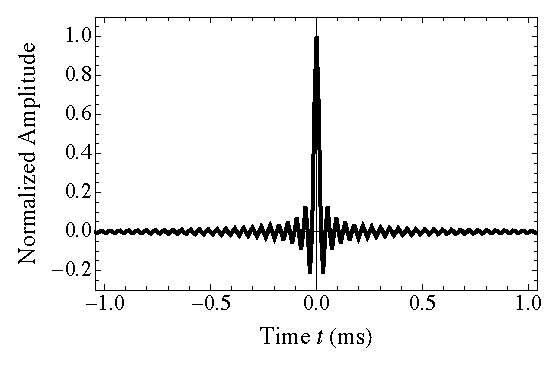
\includegraphics[width = \columnwidth]{A5_impulse_response/figures/Farina_Inverse_BPF_IR_Sm}
        \caption{Impulse response}
    \end{subfigure}
    \hfill
    \begin{subfigure}[b]{0.482\textwidth}
        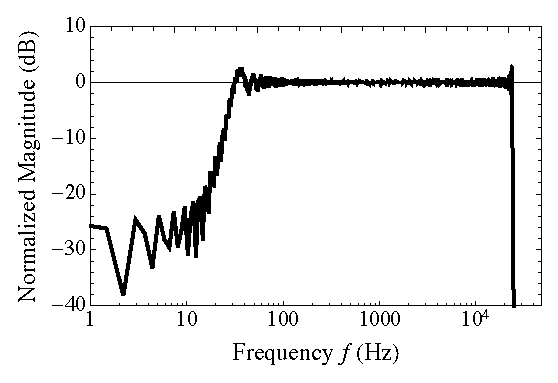
\includegraphics[width = \columnwidth]{A5_impulse_response/figures/Farina_Inverse_BPF_FR_Sm}
        \caption{Magnitude response}
    \end{subfigure}
\caption[Band-pass filter due to time-reversed deconvolution.]{
An example of the resulting band-pass filter due to time-reversed deconvolution for a $\sim23$ Hz to 24 kHz phase-controlled ESS sampled at 96 kHz.}
\label{fig:farina_BPF}
\end{figure}

For both of these deconvolution techniques, linear convolution of the recorded signal with the inverse signal is recommended to prevent part of the IR from ``wrapping around'' via cyclic convolution \citep{Farina2007a}.
The FFT can still be used, however, provided that each signal is zero-padded to at least twice its length, in which case multiplication in the frequency domain is equivalent to linear convolution in the time domain.
In our implementation, we perform exact deconvolution with appropriate zero-padding to extract the IR.

\subsection{Loudspeaker ``pop''}
One of the problems with the conventional ESS as defined in \eqnref{eq:A5_Impulse_Response:ESS} is that the loudspeaker may produce an audible ``pop'' at the end of the sweep.
This occurs when the ESS signal abruptly drops from a non-zero value to zero \citep{Farina2007a}.
The pop is undesirable as it introduces energy across the entire frequency spectrum, appearing as noise in the resulting IR.
Two solutions to this problem are to apply a time-domain fade-out to the end of the sweep \citep{Farina2007a} or to use a phase-controlled ESS up to the Nyquist frequency \citep{VetterdiRosario2011} to ensure that the sample values of the excitation signal converge more gradually towards zero.
It is worth emphasizing that the phase-controlled sweep will prevent the pop \textit{only} when terminated at the Nyquist frequency, since it is only under this condition that the samples leading up to the final sample converge towards zero.
In our implementation, we use a phase-controlled ESS and sweep up to the Nyquist frequency.

\subsection{Balancing SNR and pre-response}\label{sec:A5_Impulse_Response:Two-Step-ESS}
In view of the discussion in \secref{sec:A5_Impulse_Response:Introduction}, it is clear that knowledge of a system's pass-band may enable an improved measurement of the system's IR, as out-of-band noise may be freely attenuated via band-pass filtering without inadvertently creating a pre-response.
Motivated by this idea, a two-sweep measurement procedure was recently developed \citep{Tylka2014,Choueiri2018}, which is executed as follows:
\begin{enumerate}
\item a quick, full-band ESS is used to estimate the pass-band of the system under test,
\item a second, slower ESS through only that pass-band is used to measure the system's IR, and
\item a band-pass filter is applied to the second measurement in order to attenuate out-of-band noise.
\end{enumerate}
By matching the band-pass filter to the pass-band of the system, this method is able to attenuate out-of-band noise without introducing a significant pre-response \citep{Tylka2014}.
Additionally, the the removal of the out-of-band noise increases the overall SNR in the result of the second sweep.
In most quiet measurement environments, however, such additional steps are often unnecessary in order to achieve a reasonably high-SNR measurement without a significant pre-response.
Consequently, in our implementation, we use only single phase-controlled ESS measurements.

%\subsection{Signal-to-noise ratio}
%It has been stated that the measured SNR can be improved either by increasing the sweep duration or by averaging multiple measurements~\cite{Farina2007a,MullerMassarani2001R}.
%The latter technique, however, may lead to errors due to time-variant effects such as heating of the transducers or, in the case of outdoor measurements, wind.
%Consequently, we choose to employ a small number of longer sweeps.

\section{Summary}\label{sec:A5_Impulse_Response:Summary}
The exponential sine sweep (ESS) enables a high-SNR measurement of the impulse response of an acoustical system.
Additionally, it tends to isolate and remove a significant portion of non-linear distortion terms.
Different implementations of the ESS have been developed, and different approaches exist to extract the system's IR from the measured response (see \secref{sec:A5_Impulse_Response:ESS}).
In this appendix, we discussed issues surrounding these different approaches and, based on that discussion, we concluded that a phase-controlled ESS (see \secref{sec:A5_Impulse_Response:PC-ESS}) up to the Nyquist frequency is generally sufficient to obtain a reasonably high-SNR measurement.

\section*{Acknowledgements}
Much of this work was originally included in a presentation by \citet{Tylka2014} at the 137\textsuperscript{th} Convention of the Audio Engineering Society, along with a more detailed investigation into the recently-patented two-sweep method for measuring acoustical impulse responses, described here in \secref{sec:A5_Impulse_Response:Two-Step-ESS}.